%%%%%%%%%%%%%%%%%%%%%%%%%%%%%%%%%%%%%%%%%%%%%%%%%%%%%%%%%%%%%%%%%%%%%%%%%%%%%%%%%%%%%%%%%%%%%%%%%%%%%%%%%%%%%%%%%%%%
%%% Template de LaTeX para o Congresso Acústica 2020, que integra o XI Congreso Ibérico da Acústica, 
%%% 51º Congresso Espanhol de Acústica e TecniAcústica 2020
%%% Release 06/08/2020
%%%	Desenvolvido por Prof. William D'Andrea Fonseca da Engenharia Acústica, UFSM, Brasil
%%% will.fonseca@eac.ufsm.br
%%%%%%%%%%%%%%%%%%%%%%%%%%%%%%%%%%%%%%%%%%%%%%%%%%%%%%%%%%%%%%%%%%%%%%%%%%%%%%%%%%%%%%%%%%%%%%%%%%%%%%%%%%%%%%%%%%%%
\documentclass[11pt, a4paper, twoside]{article}
%%%%%%%%%%%%%%%%%%%%%%%%%%%%%%%%%%%%%%%%%%%%%%%%%%%%
%%% Linguagem e entrada
\usepackage[utf8]{inputenc} 
%%%%%%%%%%%%%%%%%%%%%%%%%%%%%%%%%%%%%%%%%%%%%%%%%%%%
\usepackage{ac2020}  %%% Configurações básicas do template 
%%%%%%%%%%%%%%%%%%%%%%%%%%%%%%%%%%%%%%%%%%%%%%%%%%%%%%%%%%%%%%%%%%%%%%%%%%%%%%%%%%%%%%%%%%%%%%%%%%%%%%%%%%%%%%%%%%%%
%%% Dados do artigo

\Autores{Primeiro A. Autor, Segundo B. Autor, Terceiro C. Autor} 
\AutoresFiliacoes{Primeiro A. Autor$^1$, Segundo B. Autor$^1$, Terceiro C. Autor$^2$} % Utilize números como marcadores

%% Intenta utilizar una o dos líneas como máximo para cada autor
\Filiacoes{$^1$\,Afiliação\\ \{email do primeiro autor, email do segundo autor\} \\[3pt]
$^2$\,Afiliação\\ \{email do terceiro autor\} }

\TituloCompleto{Instruções PARA A PREPARAÇÃO DE COMUNICAÇÕES PARA O\linebreak ``CONGRESSO ACÚSTICA 2020''}

\PalavrasChave{instruções, formato, regras, recomendações, no máximo 5}
\Keywords{instructions, format, rules, recommendations, maximum of 5}

\PACS{xx.xx.Nn, xx.xx.Nn}

\Resumo{O resumo deverá consistir em um ou dois parágrafos, com 6 a 10 linhas, apresentando com clareza o objetivo, principais resultados e conclusões do trabalho a apresentar. O resumo não deverá continuar na segunda página.}

\Abstract{An abstract in English should also be included. The abstract should consist of one or two paragraphs, with a total of 6 to 10 lines, clearly stating the objectives, main results and conclusions of the work. The abstract should not continue to the second page.}

%%%%%%%%%%%%%%%%%%%%%%%%%%%%%%%%%%%%%%%%%%%%%%%%%%%%%%%%%%%%%%%%%%%%%%%%%%%%%%%%%%%%%%%%%%%%%%%%%%%%%%%%%%%%%%%%%%%%
%%%%%%%%%%%%%%%%%%%%%%%%%%%%%%%%%%%%%%%%%%%%%%%%%%%%%%%%%%%%%%%%%%%%%%%%%%%%%%%%%%%%%%%%%%%%%%%%%%%%%%%%%%%%%%%%%%%%
\begin{document} \setcounter{page}{1}
%%%%%%%%%%%%%%%%%%%%%%%%%%%%%%%%%%%%%%%%%%%%%%%%%%%%%%%%%%%%%%%%%%%%%%%%%%%%%%%%%%%%%%%%%%%%%%%%%%%%%%%%%%%%%%%%%%%%
%%%%%%%%%%%%%%%%%%%%%%%%%%%%%%%%%%%%%%%%%%%%%%%%%%%%%%%%%%%%%%%%%%%%%%%%%%%%%%%%%%%%%%%%%%%%%%%%%%%%%%%%%%%%%%%%%%%%
%%% Template para de LaTeX para o evento 12º Congresso Iberoamericano de Acústica 
%%%                      em conjunto com XXIX Encontro da Sobrac
%%% Baseado no modelo da Revista Acústica e Vibrações da Sobrac
%%% Release 19/04/2022
%%%	Desenvolvido por por Prof. William D'Andrea Fonseca, Dr. Eng. - Engenharia Acústica UFSM
%%% will.fonseca@eac.ufsm.br
%%%%%%%%%%%%%%%%%%%%%%%%%%%%%%%%%%%%%%%%%%%%%%%%%%%%%%%%%%%%%%%%%%%%%%%%%%%%%%%%%%%%%%%%%%%%%%%%%%%%%%%%%%%%%%%%%%%%
%%%%%%%%%%%%%%%%%%%%%%%%%%%%%%%%%%%%%%%%%%%%%%%%%%%%%%%%%%%%%%%%%%%%%%%%%%%%%%%%%%%%%%%%%%%%%%%%%%%%%%%%%%%%%%%%%%%%
%% Estilo do artigo
\pagestyle{plain}
%%%%%%%%%%%%%%%%%%%%%%%%%%%%%%%%%%%%%%%%%%%%%%%%%%%%%%%%%%%%%%%%%%%%%%%%%%%%%%%%%%%%%%%%%%%%%%%%%%%%%%%%%%%%%%%%%%%%
%%% Primeira página
\thispagestyle{firststyle}
% \newgeometry{top=2.1cm, bottom=2cm, left=1.9cm, right=1.9cm, headsep=5mm}
%%%%%%%%%%%%%%%%%%%%%%%%%%%%%%%%%%%%%%%%%%%%%%%%%%%%%%%%%%%%%%%%%%%%%%%%%%%%%%%%%%%%%%%%%%%%%%%%%%%%%%%%%%%%%%%%%%%%
\begin{textblock}{200}(150.2,283.51)
\fontsize{8}{8}\selectfont\sffamily 
DOI:~\href{https://doi.org/\DOIArtigo}{\DOIArtigo}
\end{textblock}
%%% Título
\begin{textblock}{170}(37,12)

\includegraphics[width=0.82\textwidth,page=1]{FIA-logo.pdf}
\end{textblock}

\twocolumn[
\begin{@twocolumnfalse}
\vspace{60pt}
\begin{center}
{\fontsize{18}{22}\selectfont\bfseries 
%% Título
%%%%%%%%%%%%%%%%%%%%%%%%%%%%%%%%%%%%%%%%%%%%%%%%%%%%%%%%%%%%%%%%%%%%%%%%%%%%%%%%%%%%%%%%%%%%%%%%%%%%%%%%%%%%%%%%%%%%
\TituloCompletoArtigo \bookmark[page=1,level=1]{Título e Resumo}
%%%%%%%%%%%%%%%%%%%%%%%%%%%%%%%%%%%%%%%%%%%%%%%%%%%%%%%%%%%%%%%%%%%%%%%%%%%%%%%%%%%%%%%%%%%%%%%%%%%%%%%%%%%%%%%%%%%%
\par}

%%%%%%%%%%%%%%%%%%%%%%%%%%%%%%%%%%%%%%%%%%%%%%%%%%%%%%%%%%%%%%%%%%%%%%%%%%%%%%%%%%%%%%%%%%%%%%%%%%%%%%%%%%%%%%%%%%%
%%%%%%%%%%%%%%%%%%%%%%%%%%%%%%%%%%%%%%%%%%%%%%%%%%%%%%%%%%%%%%%%%%%%%%%%%%%%%%%%%%%%%%%%%%%%%%%%%%%%%%%%%%%%%%%%%%%
\vspace{12pt}
{\fontsize{11}{13}\selectfont \bfseries 
%% Autores
%%%%%%%%%%%%%%%%%%%%%%%%%%%%%%%%%%%%%%%%%%%%%%%%%%%%%%%%%%%%%%%%%%%%%%%%%%%%%%%%%%%%%%%%%%%%%%%%%%%%%%%%%%%%%%%%%%%
\AutoresFiliacoesArtigo
%%%%%%%%%%%%%%%%%%%%%%%%%%%%%%%%%%%%%%%%%%%%%%%%%%%%%%%%%%%%%%%%%%%%%%%%%%%%%%%%%%%%%%%%%%%%%%%%%%%%%%%%%%%%%%%%%%%
\par}

\vspace{2mm}
{\fontsize{9}{11}\selectfont 
%% Filiações
%%%%%%%%%%%%%%%%%%%%%%%%%%%%%%%%%%%%%%%%%%%%%%%%%%%%%%%%%%%%%%%%%%%%%%%%%%%%%%%%%%%%%%%%%%%%%%%%%%%%%%%%%%%%%%%%%%%
\FiliacoesArtigo
%%%%%%%%%%%%%%%%%%%%%%%%%%%%%%%%%%%%%%%%%%%%%%%%%%%%%%%%%%%%%%%%%%%%%%%%%%%%%%%%%%%%%%%%%%%%%%%%%%%%%%%%%%%%%%%%%%%%
\par}
\end{center}

\vspace{-5mm}{\color{FIABlue}\rule{\textwidth}{0.4pt}}
%%%%%%%%%%%%%%%%%%%%%%%%%%%%%%%%%%%%%%%%%%%%%%%%%%%%%%%%%%%%%%%%%%%%%%%%%%%%%%%%%%%%%%%%%%%%%%%%%%%%%%%%%%%%%%%%%%%%
%%%%%%%%%%%%%%%%%%%%%%%%%%%%%%%%%%%%%%%%%%%%%%%%%%%%%%%%%%%%%%%%%%%%%%%%%%%%%%%%%%%%%%%%%%%%%%%%%%%%%%%%%%%%%%%%%%%%
%%% Resumo e palavras-chave
\ResumoTexto
%%%%%%%%%%%%%%%%%%%%%%%%%%%%%%%%%%%%%%%%%%%%%%%%%%%%%%%%%%%%%
%%% Title, abstract and keywords
%%%%%%%%%%%%%%%%%%%%%%%%%%%%%%%%%%%%%%%%%%%%%%%%%%%%%%%%%%%%%
%%% Title
\begin{otherlanguage*}{english}
{\EnglishTitle}
%%%%%%%%%%%%%%%%%%%%%%%%%%%%%%%%%%%%%%%%%%%%%%%%%%%%%%%%%%%%%%%%%%%%%%%%%%%%%%%%%%%%%%%%%%%%%%%%%%%%%%%%%%%%%%%%%%%%
%%%%%%%%%%%%%%%%%%%%%%%%%%%%%%%%%%%%%%%%%%%%%%%%%%%%%%%%%%%%%%%%%%%%%%%%%%%%%%%%%%%%%%%%%%%%%%%%%%%%%%%%%%%%%%%%%%%%
%%% Abstract
		{\textbf{Abstract}} \vspace{5pt}
		
		{\fontsize{11}{12.5}\selectfont
		\AbstractArtigo
		\par}
		%%%%%%%%%%%%%%%%%%%%%%%%% Keywords
		\vspace{0.7\baselineskip} \fontsize{11}{12}\selectfont
		\textbf{Keywords: }{\fontsize{11}{12}\selectfont 
		\KeywordsArtigo.
		\par}
		%%%%%%%%%%%%%%%%%%%%%%%%% PACs:
		\PACSEnglish
	  \vspace{6mm}
\end{otherlanguage*}		
%%%%%%%%%%%%%%%%%%%%%%%%%%%%%%%%%%%%%%%%%%%%%%%%%%%%%%%%%%%%%%%%%%%%%%%%%%%%%%%%%%%%%%%%%%%%%%%%%%%%%%%%%%%%%%%%%%%%
%%%%%%%%%%%%%%%%%%%%%%%%%%%%%%%%%%%%%%%%%%%%%%%%%%%%%%%%%%%%%%%%%%%%%%%%%%%%%%%%%%%%%%%%%%%%%%%%%%%%%%%%%%%%%%%%%%%%
\end{@twocolumnfalse}
]
% \restoregeometry 
% \newgeometry{top=2.1cm, bottom=2cm, left=1.9cm, right=1.9cm, headsep=5mm}
\pagestyle{plain}

%%%%%%%%%%%%%%%%%%%%%%%%%%%%%%%%%%%%%%%%%%%%%%%%%%%%%%%%%%%%%%%%%%%%%%%%%%%%%%%%%%%%%%%%%%%%%%%%%%%%%%%%%%%%%%%%%%%%
% EOF

%%%%%%%%%%%%%%%%%%%%%%%%%%%%%%%%%%%%%%%%%%%%%%%%%%%%%%%%%%%%%%%%%%%%%%%%%%%%%%%%%%%%%%%%%%%%%%%%%%%%%%%%%%%%%%%%%%%%
%%%%%%%%%%%%%%%%%%%%%%%%%%%%%%%%%%%%%%%%%%%%%%%%%%%%%%%%%%%%%%%%%%%%%%%%%%%%%%%%%%%%%%%%%%%%%%%%%%%%%%%%%%%%%%%%%%%%
%%% ARTIGO
%%%%%%%%%%%%%%%%%%%%%%%%%%%%%%%%%%%%%%%%%%%%%%%%%%%%%%%%%%%%%%%%%%%%%%%%%%%%%%%%%%%%%%%%%%%%%%%%%%%%%%%%%%%%%%%%%%%%
%%%%%%%%%%%%%%%%%%%%%%%%%%%%%%%%%%%%%%%%%%%%%%%%%%%%%%%%%%%%%%%%%%%%%%%%%%%%%%%%%%%%%%%%%%%%%%%%%%%%%%%%%%%%%%%%%%%%
\section{Introdução}

Este documento constitui o template/modelo a seguir na preparação dos artigos para o Congresso Acústica 2020. Note-se que é necessário incluir as referências PACS (Physics and Astronomy Classification Scheme) respeitantes aos tópicos a que o artigo diz respeito. A listagem completa destas referências pode ser obtida a partir do website da SEA (\url{http://www.sea-acustica.es/?id=46}).


%%%%%%%%%%%%%%%%%%%%%%%%%%%%%%%%%%%%%%%%%%%%%%%%%%%%%%%%%%%%%%%%%%%%%%%%%%%%%%%%%%%%%%%%%%%%%%%%%%%%%%%%%%%%%%%%%%%%
%%%%%%%%%%%%%%%%%%%%%%%%%%%%%%%%%%%%%%%%%%%%%%%%%%%%%%%%%%%%%%%%%%%%%%%%%%%%%%%%%%%%%%%%%%%%%%%%%%%%%%%%%%%%%%%%%%%%
\section{Submissão e publicação}

Nesta seção são apresentados os detalhes para a submissão.

%%%%%%%%%%%%%%%%%%%%%%%%%%%%%%%%%%%%%%%%%%%%%%%%%%%%%%%%%%%%%%%%%%%%%%%%%%%%%%%%%%%%%%%%%%%%%%%%%%%%%%%%
\subsection{Submissão das comunicações}

As comunicações deverão ser submetidas de forma eletrónica (em formato PDF), por meio do website do Congresso em \url{http://www.spacustica.pt/acustica2020/index.html}. 

\clearpage
%%%%%%%%%%%%%%%%%%%%%%%%%%%%%%%%%%%%%%%%%%%%%%%%%%%%%%%%%%%%%%%%%%%%%%%%%%%%%%%%%%%%%%%%%%%%%%%%%%%%%%%%%%%%%%%%%%%%
%%%%%%%%%%%%%%%%%%%%%%%%%%%%%%%%%%%%%%%%%%%%%%%%%%%%%%%%%%%%%%%%%%%%%%%%%%%%%%%%%%%%%%%%%%%%%%%%%%%%%%%%%%%%%%%%%%%%
\section{Regras gerais de formatação}

Na formatação dos artigos deve ser seguido o template/modelo apresentado neste documento. 
A comunicação não deverá exceder as 12 páginas (A4). O tamanho máximo do ficheiro não deverá exceder os 5~MB.


%%%%%%%%%%%%%%%%%%%%%%%%%%%%%%%%%%%%%%%%%%%%%%%%%%%%%%%%%%%%%%%%%%%%%%%%%%%%%%%%%%%%%%%%%%%%%%%%%%%%%%%%
\subsection{Formatação do texto}

Nesta seção detalhes de formatação são apresentados.


%%%%%%%%%%%%%%%%%%%%%%%%%%%%%%%%%%%%%%%%%%%%%%%%%%%%%%%%%%%%%%%%%%%%%%%%%%%%%%%%%%%%%%%%%%%%%%%%%%%%%%%%
\subsubsection{Tabelas e figuras}

As tabelas e as figuras deverão ser centradas, numeradas de forma consecutiva e apresentar uma legenda descritiva centrada na página (ver, por exemplo, a \tabela{tab.exemplo} e a \Figura{fig:beamforming}).

\begin{table}[H]
  \centering 
  \caption{Exemplo de tabela xxx / yyy.}
	\fontsize{11}{12}\selectfont 
    \begin{tabular}{C{2.8cm} | C{2.8cm}}
    \toprule
		\SetRowColor{LightOrange}
    \textbf{ xxx } & \textbf{yyy} \\
	  \midrule
		10 & 3120\\
		\rowcolor[gray]{.95} 40	& 2555\\
		50 & 1100\\
    \bottomrule
    \end{tabular}
    \label{tab.exemplo}%
\end{table}%


\begin{figure}[H]
	\centering
	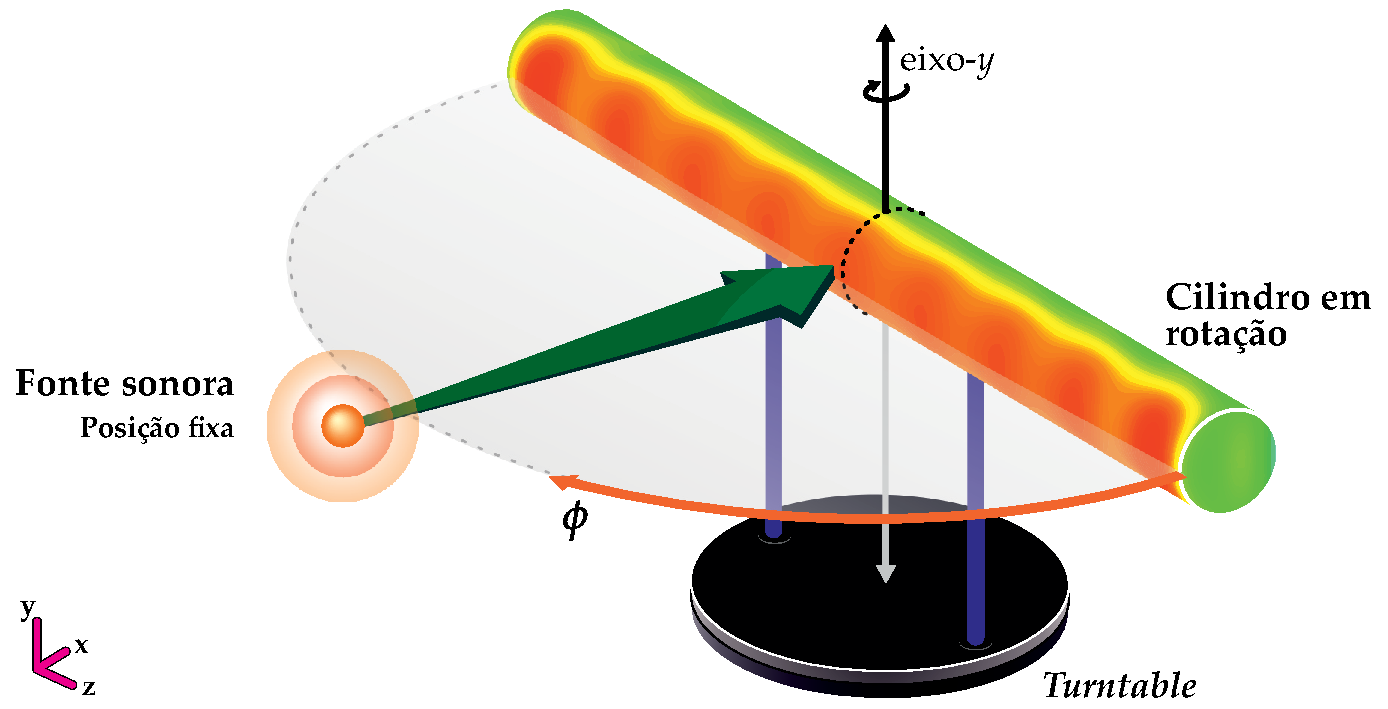
\includegraphics[width=0.75\linewidth]{Figuras/Measurement-Scheme-Fonseca-2013.pdf}%
	\caption{Exemplo de figura com legenda (adaptado de Fonseca \cite{Fonseca-2013}).}%
	\label{fig:beamforming}%
\end{figure}


%%%%%%%%%%%%%%%%%%%%%%%%%%%%%%%%%%%%%%%%%%%%%%%%%%%%%%%%%%%%%%%%%%%%%%%%%%%%%%%%%%%%%%%%%%%%%%%%%%%%%%%%
\subsubsection{Equações}

As equações deverão ser numeradas sequencialmente, utilizando caracteres árabes entre parênteses. As expressões deverão ser centradas, deixando espaços de 6 pt acima e abaixo, para separá-las do resto do texto. A título de exemplo, considere 
%
\begin{equation}
Ax = b \,,
\label{eq:eq1}
\end{equation}
%
em que $A$ e $b$ são constantes. Deverão ser utilizados símbolos convencionais e unidades SI. 


%%%%%%%%%%%%%%%%%%%%%%%%%%%%%%%%%%%%%%%%%%%%%%%%%%%%%%%%%%%%%%%%%%%%%%%%%%%%%%%%%%%%%%%%%%%%%%%%%%%%%%%%
\subsection{Citação de referências}

Ao longo do texto, as referências bibliográficas deverão ser citadas utilizando números entre parênteses rectos \cite{Fonseca-2013,ref2,TADEU2006,ref4,refBranco,ref6,Brebbia}. Na seção de referências, sempre que possível, inclua o ISBN, DOI (com link) e/ou link com a direção online em que o documento citado está disponível.

%%%%%%%%%%%%%%%%%%%%%%%%%%%%%%%%%%%%%%%%%%%%%%%%%%%%%%%%%%%%%%%%%%%%%%%%%%%%%%%%%%%%%%%%%%%%%%%%%%%%%%%%%%%%%%%%%%%%%%%%%%%%%%%%%%%%%%%%%%%%%%%%%%%%%%%%%%%%%%%%%%%%%%%%%%%%%%%%%%%%%%%%%%
\section{Conclusões}

Pelo menos um dos autores deverá inscrever se e regularizar o correspondente pagamento, para que a comunicação seja aceita para apresentação no Congresso e publicação nas respetivas Atas.

%%%%%%%%%%%%%%%%%%%%%%%%%%%%%%%%%%%%%%%%%%%%%%%%%%%%%%%%%%%%%%%%%%%%%%%%%%%%%%%%%%%%%%%%%%%%%%%%%%%%%%%%%%%%%%%%%%%%%%%%%%%%%%%%%%%%%%%%%%%%%%%%%%%%%%%%%%%%%%%%%%%%%%%%%%%%%%%%%%%%%%%%%%
\subsection*{Agradecimentos}

Agradecimentos ou alusão a pessoas ou entidades deverão ser colocados no final do texto, em secção própria, antes da secção das referências.

%%%%%%%%%%%%%%%%%%%%%%%%%%%%%%%%%%%%%%%%%%%%%%%%%%%%%%%%%%%%%%%%%%%%%%%%%%%%%%%%%%%%%%%%%%%%%%%%%%%%%%%%%%%%%%%%%%%%
%%%%%%%%%%%%%%%%%%%%%%%%%%%%%%%%%%%%%%%%%%%%%%%%%%%%%%%%%%%%%%%%%%%%%%%%%%%%%%%%%%%%%%%%%%%%%%%%%%%%%%%%%%%%%%%%%%%%
%%% Referências
\renewcommand{\refname}{Referências} 
\bibliographystyle{unsrtnat2}
\bibliography{bibliografia}
%%%%%%%%%%%%%%%%%%%%%%%%%%%%%%%%%%%%%%%%%%%%%%%%%%%%%%%%%%%%%%%%%%%%%%%%%%%%%%%%%%%%%%%%%%%%%%%%%%%%%%%%
%%%%%%%%%%%%%%%%%%%%%%%%%%%%%%%%%%%%%%%%%%%%%%%%%%%%%%%%%%%%%%%%%%%%%%%%%%%%%%%%%%%%%%%%%%%%%%%%%%%%%%%%
\end{document}
% EOF %%%%%%%%%%%%%%%%%%%%%%%%%%%%%%%%%%%%%%%%%%%%%%%%%%%%%%%%%%%%%%%%%%%%%%%%%%%%%%%%%%%%%%%%%%%%%%%%%%